\documentclass[sigconf]{acmart}

\usepackage{booktabs} % For formal tables
\usepackage{graphicx}
\usepackage{rotating}
\usepackage{tabularx}
\usepackage{xstring} % for string operations
\usepackage{wasysym} % Table legend with symbols input from post-processing
\usepackage{MnSymbol} % Table legend with symbols input from post-processing
\usepackage{float}

% define some COCO/dvipsnames colors
\definecolor{Gray}{gray}{0.6}
\definecolor{NavyBlue}{rgb}{0.0, 0.0, 0.5}
\definecolor{Magenta}{rgb}{1.0, 0.0, 1.0}
\definecolor{Black}{rgb}{0.0, 0.0, 0.0}

%%%%%%%%%%%%%%%%%%%%%%%%%%%%%%%%%%%%%%%%%%%%%%%%%%%%%%
% Packages
%\usepackage{graphicx}
%\usepackage[dvipsnames]{xcolor}
%\usepackage{float}
%\usepackage{xstring} % for string operations
%\usepackage{wasysym} % Table legend with symbols input from post-processing
%\usepackage{MnSymbol} % Table legend with symbols input from post-processing
%\usepackage[colorlinks=true, linkcolor=blue]{hyperref} % make COCO papers clickable




% Copyright
%\setcopyright{none}
%\setcopyright{acmcopyright}
%\setcopyright{acmlicensed}
\setcopyright{rightsretained}
%\setcopyright{usgov}
%\setcopyright{usgovmixed}
%\setcopyright{cagov}
%\setcopyright{cagovmixed}


% DOI
\acmDOI{10.475/123_4}

% ISBN
\acmISBN{123-4567-24-567/08/06}

%Conference
\acmConference[GECCO '17]{the Genetic and Evolutionary Computation Conference 2017}{July 15--19, 2017}{Berlin, Germany}
\acmYear{2017}
\copyrightyear{2017}

\acmPrice{15.00}



%%%%%%%%%%%%%%%%%%%%%%   END OF PREAMBLE   %%%%%%%%%%%%%%%%%%%%%%%%%%%%%%%%%%%%

%%%%%%%%%%%%%%%%%%%%%%%%%%%%%%%%%%%%%%%%%%%%%%%%%%%%%%%%%%%%%%%%%%%%%%%%%%%%%%%
%%%%%%%%% TO BE EDITED %%%%%%%%%%%%%%%%%%%%%%%%%%%%%%%%%%%%%%%%%%%%%%%%%%%%%%%%
%%%%%%%%%%%%%%%%%%%%%%%%%%%%%%%%%%%%%%%%%%%%%%%%%%%%%%%%%%%%%%%%%%%%%%%%%%%%%%%
% specify acronyms for algorithm1 (1st arg. of post-processing) and algorithm2 (2nd arg.) 
%\newcommand{\algorithmA}{algorithmB}  % first argument in the post-processing
%\newcommand{\algorithmB}{algorithmB}  % second argument in the post-processing
% for the short acronyms in the tables, adjust the following to lines if required.
%\newcommand{\algorithmAshort}{algA}  % first argument in the post-processing
%\newcommand{\algorithmBshort}{algB}  % second argument in the post-processing

% rungeneric.py writes data into a subfolder of ppdata
\newcommand{\bbobdatapath}{ppdata/} % change default output folder of COCO if desired
\input{\bbobdatapath cocopp_commands.tex} % provide default of algname and algfolder
%%%%%%%%%%%%%%%%%%%%%%%%%%%%%%%%%%%%%%%%%%%%%%%%%%%%%%%%%%%%%%%%%%%%%%%%%%%%%%%
%%%%%%%%%%%%%%%%%%%%%%%%%%%%%%%%%%%%%%%%%%%%%%%%%%%%%%%%%%%%%%%%%%%%%%%%%%%%%%%
%%%%%%%%%%%%%%%%%%%%%%%%%%%%%%%%%%%%%%%%%%%%%%%%%%%%%%%%%%%%%%%%%%%%%%%%%%%%%%%
\graphicspath{{\bbobdatapath}}

% pre-defined commands
\newcommand{\DIM}{\ensuremath{\mathrm{DIM}}}
\newcommand{\aRT}{\ensuremath{\mathrm{aRT}}}
\newcommand{\FEvals}{\ensuremath{\mathrm{FEvals}}}
\newcommand{\nruns}{\ensuremath{\mathrm{Nruns}}}
\newcommand{\Dfb}{\ensuremath{\Delta f_{\mathrm{best}}}}
\newcommand{\Df}{\ensuremath{\Delta f}}
\newcommand{\nbFEs}{\ensuremath{\mathrm{\#FEs}}}
\newcommand{\fopt}{\ensuremath{f_\mathrm{opt}}}
\newcommand{\ftarget}{\ensuremath{f_\mathrm{t}}}
\newcommand{\CrE}{\ensuremath{\mathrm{CrE}}}
\newcommand{\change}[1]{{\color{red} #1}}


\begin{document}

\title{Black-Box Optimization Benchmarking Template for the Comparison of Two Algorithms on the Noiseless Testbed}
\renewcommand{\shorttitle}{Black-Box Optimization Benchmarking Template for Two Algorithms}
\titlenote{Submission deadline: March 31st.}
%Camera-ready paper due April 24th.}}
\subtitle{Draft version}



\author{Firstname Lastname}
%\authornote{tba if needed}
%\orcid{1234-5678-9012}
%\affiliation{%
%  \institution{Institute for Clarity in Documentation}
%  \streetaddress{P.O. Box 1212}
%  \city{Dublin} 
%  \state{Ohio} 
%  \postcode{43017-6221}
%}
%\email{trovato@corporation.com}
%
%\author{G.K.M. Tobin}
%\authornote{The secretary disavows any knowledge of this author's actions.}
%\affiliation{%
%  \institution{Institute for Clarity in Documentation}
%  \streetaddress{P.O. Box 1212}
%  \city{Dublin} 
%  \state{Ohio} 
%  \postcode{43017-6221}
%}
%\email{webmaster@marysville-ohio.com}
%
%\author{Lars Th{\o}rv{\"a}ld}
%\authornote{This author is the
%  one who did all the really hard work.}
%\affiliation{%
%  \institution{The Th{\o}rv{\"a}ld Group}
%  \streetaddress{1 Th{\o}rv{\"a}ld Circle}
%  \city{Hekla} 
%  \country{Iceland}}
%\email{larst@affiliation.org}
%
%\author{Lawrence P. Leipuner}
%\affiliation{
%  \institution{Brookhaven Laboratories}
%  \streetaddress{P.O. Box 5000}}
%\email{lleipuner@researchlabs.org}
%
%\author{Sean Fogarty}
%\affiliation{%
%  \institution{NASA Ames Research Center}
%  \city{Moffett Field}
%  \state{California} 
%  \postcode{94035}}
%\email{fogartys@amesres.org}
%
%\author{Charles Palmer}
%\affiliation{%
%  \institution{Palmer Research Laboratories}
%  \streetaddress{8600 Datapoint Drive}
%  \city{San Antonio}
%  \state{Texas} 
%  \postcode{78229}}
%\email{cpalmer@prl.com}
%
%\author{John Smith}
%\affiliation{\institution{The Th{\o}rv{\"a}ld Group}}
%\email{jsmith@affiliation.org}
%
%\author{Julius P.~Kumquat}
%\affiliation{\institution{The Kumquat Consortium}}
%\email{jpkumquat@consortium.net}

% The default list of authors is too long for headers}
\renewcommand{\shortauthors}{Firstname Lastname et. al.}


\begin{abstract}
to be written
\end{abstract}


%
% The code below should be generated by the tool at
% http://dl.acm.org/ccs.cfm
% Please copy and paste the code instead of the example below. 
%
 \begin{CCSXML}
<ccs2012>
<concept>
<concept_id>10010147.10010178.10010205.10010208</concept_id>
<concept_desc>Computing methodologies~Continuous space search</concept_desc>
<concept_significance>500</concept_significance>
</concept>
</ccs2012>
\end{CCSXML}

\ccsdesc[500]{Computing methodologies~Continuous space search}


% We no longer use \terms command
%\terms{Algorithms}

% Complete with anything that is needed
\keywords{Benchmarking, Black-box optimization}

\maketitle


% \section{Introduction}
%
% \section{Algorithm Presentation}
%
% \section{Experimental Procedure}
%
%%%%%%%%%%%%%%%%%%%%%%%%%%%%%%%%%%%%%%%%%%%%%%%%%%%%%%%%%%%%%%%%%%%%%%%%%%%%%%%
\section{CPU Timing}
%%%%%%%%%%%%%%%%%%%%%%%%%%%%%%%%%%%%%%%%%%%%%%%%%%%%%%%%%%%%%%%%%%%%%%%%%%%%%%%
% note that the following text is just a proposal and can/should be changed to your needs:
In order to evaluate the CPU timing of the algorithm, we have run the \change{MY-ALGORITHM-NAME} on the  \change{bbob test suite \cite{hansen2010fun}} with restarts for a maximum budget equal to \change{$400 (D + 2)$} function evaluations according to \cite{hansen2016exp}. The \change{C/Java/Python/Matlab/Octave} code was run on a \change{Mac Intel(R) Core(TM) i5-2400S CPU @ 2.50GHz} with \change{1} processor and \change{4} cores \change{and (compile) options xxx}. The time per function evaluation for dimensions 2, 3, 5, 10, 20\change{, 40} equals \change{$x.x$}, \change{$x.x$}, \change{$x.x$}, \change{$xx$}, \change{$xxx$}\change{, and $xxx$} seconds respectively. 

\change{repeat the above for the second algorithm}

%%%%%%%%%%%%%%%%%%%%%%%%%%%%%%%%%%%%%%%%%%%%%%%%%%%%%%%%%%%%%%%%%%%%%%%%%%%%%%%
\section{Results}
%%%%%%%%%%%%%%%%%%%%%%%%%%%%%%%%%%%%%%%%%%%%%%%%%%%%%%%%%%%%%%%%%%%%%%%%%%%%%%%

Results from experiments according to \cite{hansen2016exp} and \cite{hansen2016perfass} on the benchmark
functions given in \cite{wp200901_2010,hansen2010fun} are presented in
Figures~\ref{fig:scaling}, \ref{fig:scatterplots} and \ref{fig:RLDs} and
in Table~\ref{tab:aRTs}. The experiments were performed with COCO \cite{hansen2016cocoplat},
version \change{2.0}, the plots were produced with version \change{2.0}.

The \textbf{average runtime (aRT)}, used in the figures and table, depends on a
given target function value, $\ftarget=\fopt+\Df$, and is computed over all relevant trials
as the number of function evaluations executed during each trial while the best
function value did not reach \ftarget, summed over all trials
and divided by the number of trials that actually reached \ftarget\
\cite{hansen2010exp,price1997dev}.
\textbf{Statistical significance} is tested with the rank-sum test for a given
target $\Delta\ftarget$ ($10^{-8}$ as in Figure~\ref{fig:scaling}) using,
for each trial, either the number of needed function evaluations to reach
$\Delta\ftarget$ (inverted and multiplied by $-1$), or, if the target was not
reached, the best $\Df$-value achieved, measured only up to the smallest number
of overall function evaluations for any unsuccessful trial under consideration.


%%%%%%%%%%%%%%%%%%%%%%%%%%%%%%%%%%%%%%%%%%%%%%%%%%%%%%%%%%%%%%%%%%%%%%%%%%%%%%%
%%%%%%%%%%%%%%%%%%%%%%%%%%%%%%%%%%%%%%%%%%%%%%%%%%%%%%%%%%%%%%%%%%%%%%%%%%%%%%%

% Scaling of aRT with dimension

%%%%%%%%%%%%%%%%%%%%%%%%%%%%%%%%%%%%%%%%%%%%%%%%%%%%%%%%%%%%%%%%%%%%%%%%%%%%%%%
\begin{figure*}
\centering
\begin{tabular}{@{}c@{}c@{}c@{}c@{}}
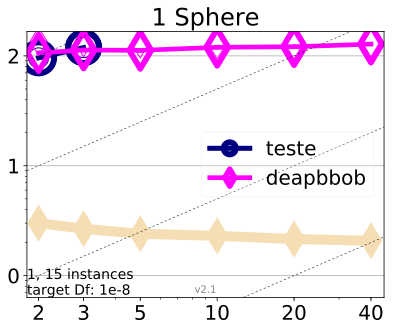
\includegraphics[width=0.253\textwidth, trim= 0.7cm 0.8cm 0.5cm 0.5cm, clip]{ppfigs_f001}&
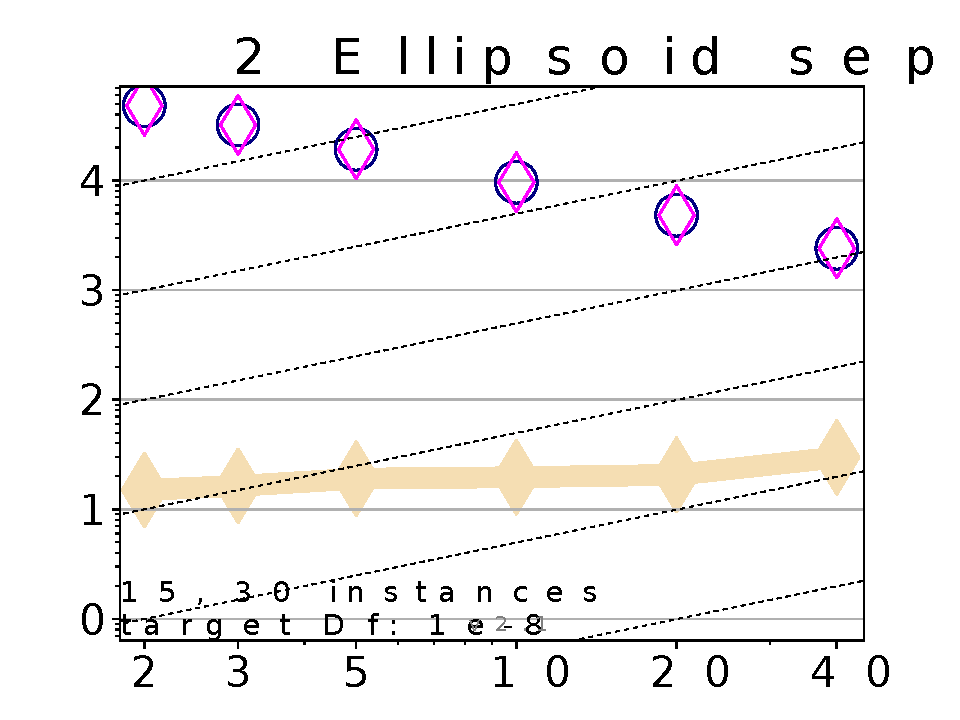
\includegraphics[width=0.238\textwidth, trim= 1.8cm 0.8cm 0.5cm 0.5cm, clip]{ppfigs_f002}&
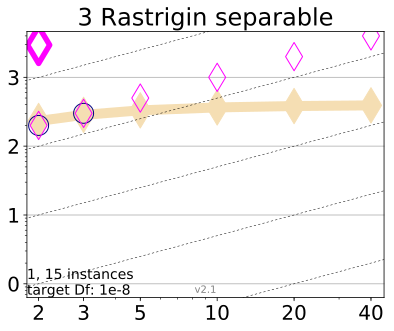
\includegraphics[width=0.238\textwidth, trim= 1.8cm 0.8cm 0.5cm 0.5cm, clip]{ppfigs_f003}&
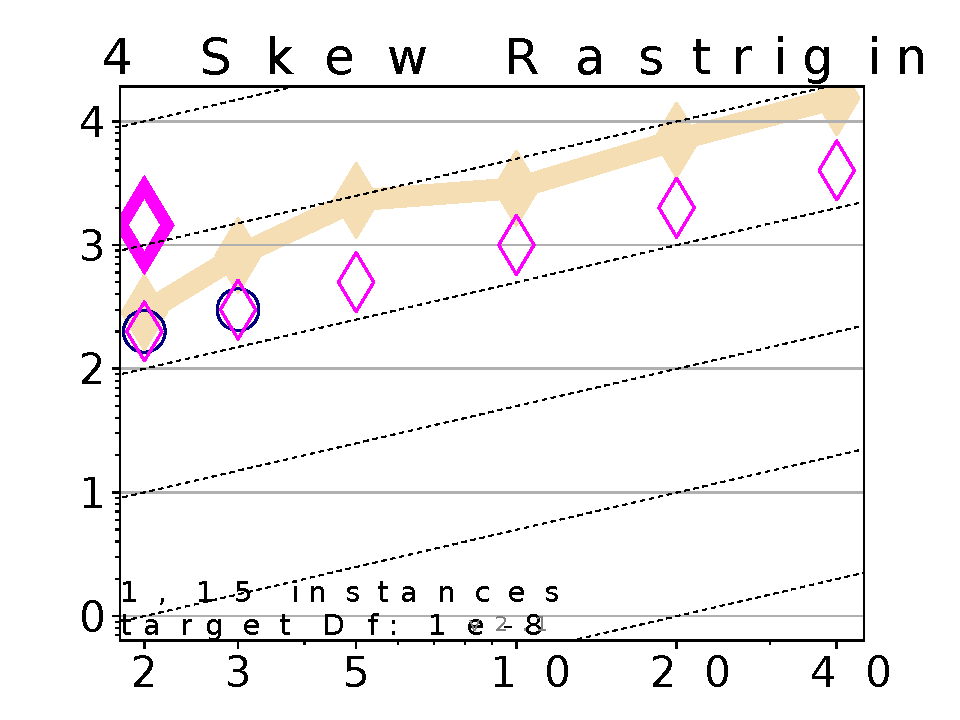
\includegraphics[width=0.238\textwidth, trim= 1.8cm 0.8cm 0.5cm 0.5cm, clip]{ppfigs_f004}\\
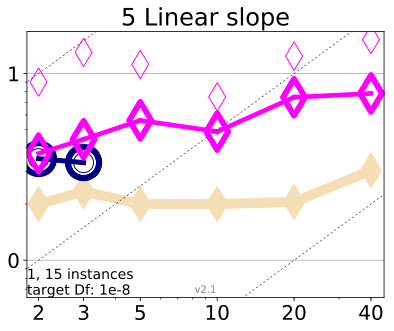
\includegraphics[width=0.253\textwidth, trim= 0.7cm 0.8cm 0.5cm 0.5cm, clip]{ppfigs_f005}&
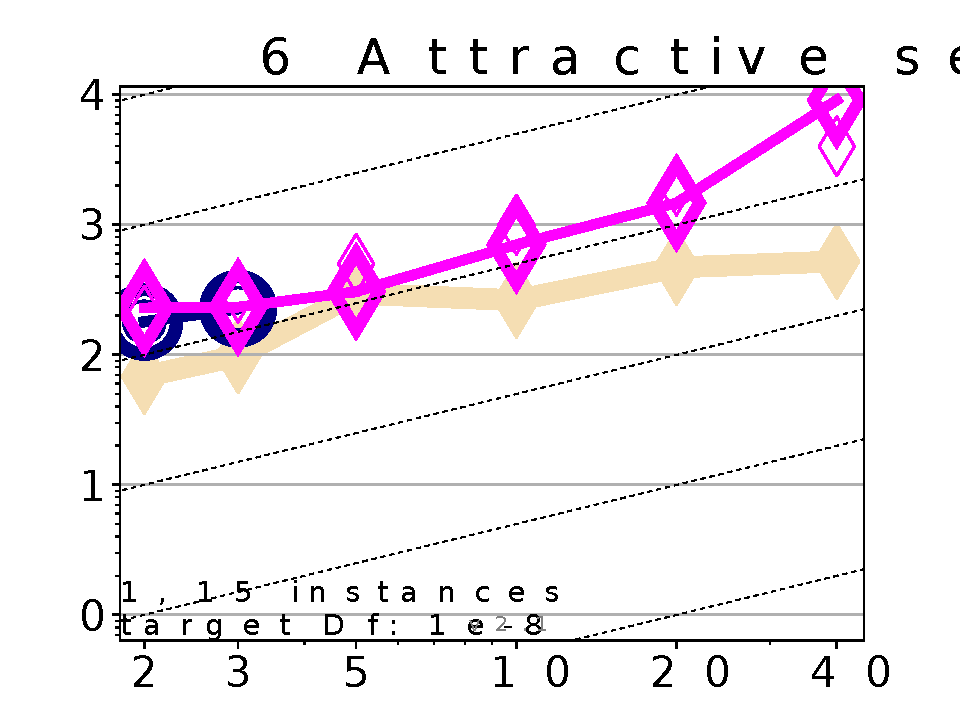
\includegraphics[width=0.238\textwidth, trim= 1.8cm 0.8cm 0.5cm 0.5cm, clip]{ppfigs_f006}&
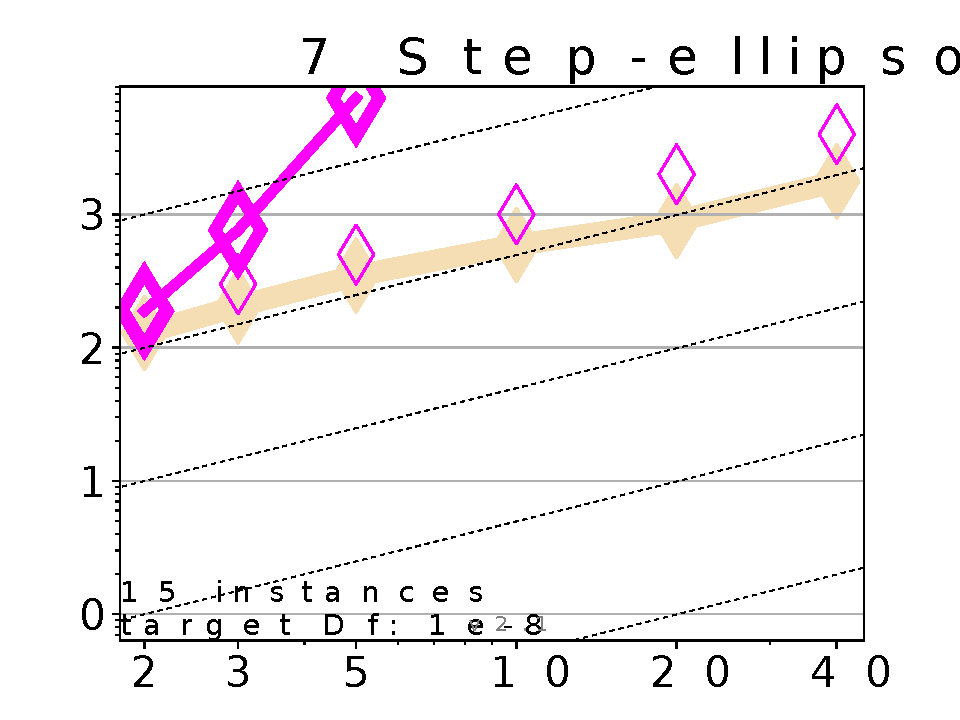
\includegraphics[width=0.238\textwidth, trim= 1.8cm 0.8cm 0.5cm 0.5cm, clip]{ppfigs_f007}&
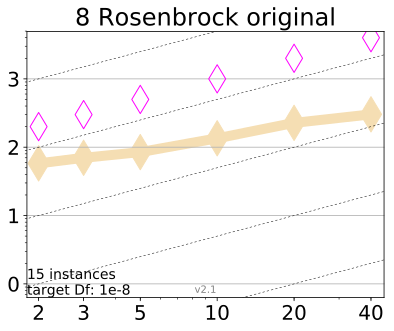
\includegraphics[width=0.238\textwidth, trim= 1.8cm 0.8cm 0.5cm 0.5cm, clip]{ppfigs_f008}\\
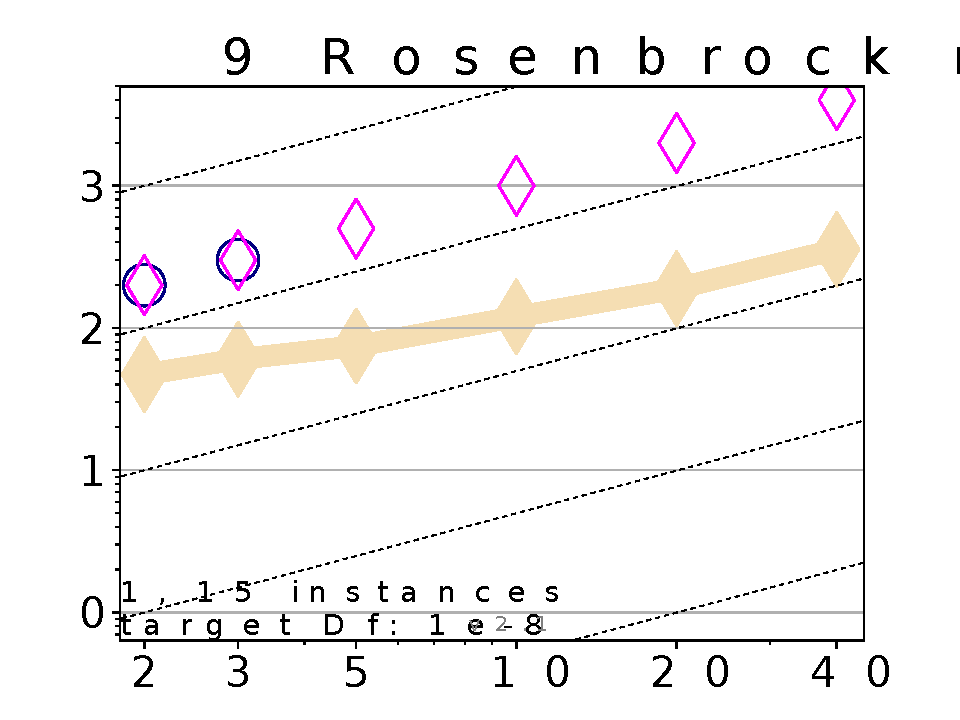
\includegraphics[width=0.253\textwidth, trim= 0.7cm 0.8cm 0.5cm 0.5cm, clip]{ppfigs_f009}&
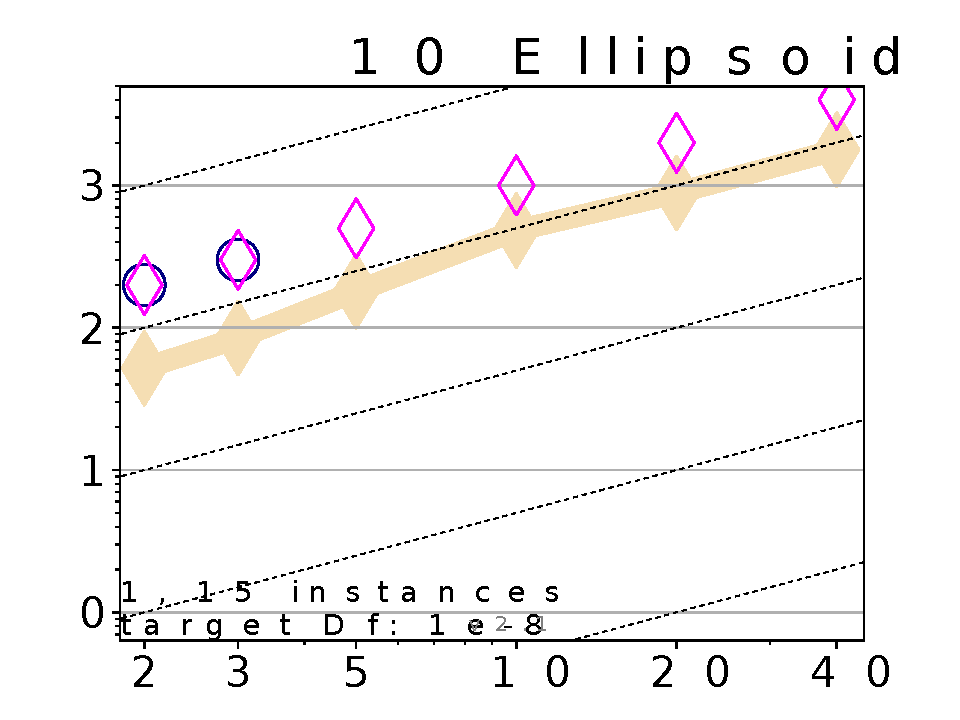
\includegraphics[width=0.238\textwidth, trim= 1.8cm 0.8cm 0.5cm 0.5cm, clip]{ppfigs_f010}&
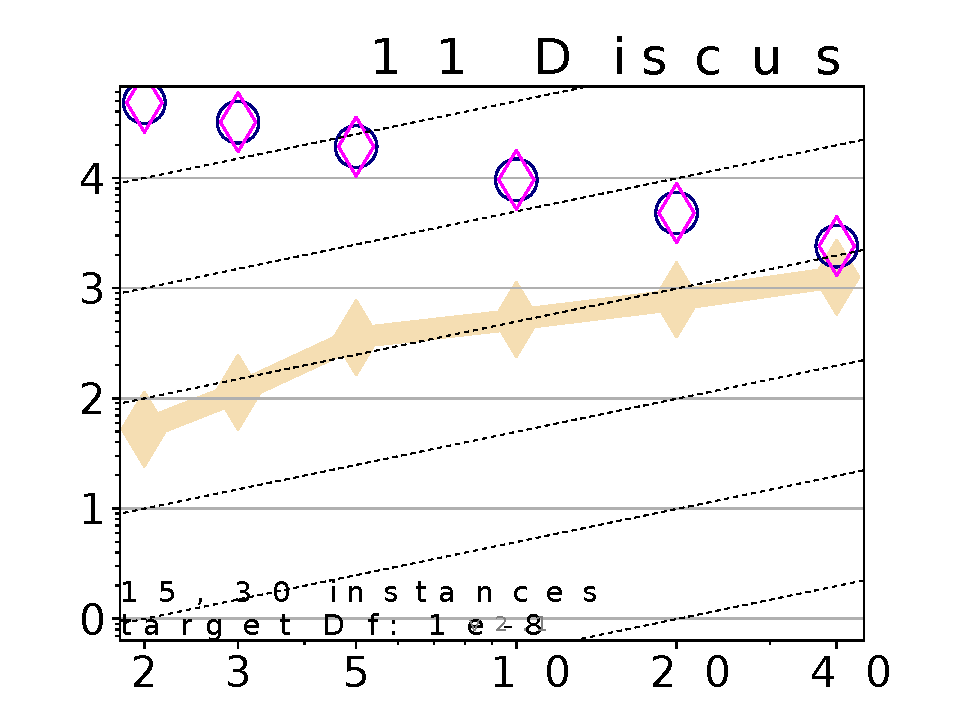
\includegraphics[width=0.238\textwidth, trim= 1.8cm 0.8cm 0.5cm 0.5cm, clip]{ppfigs_f011}&
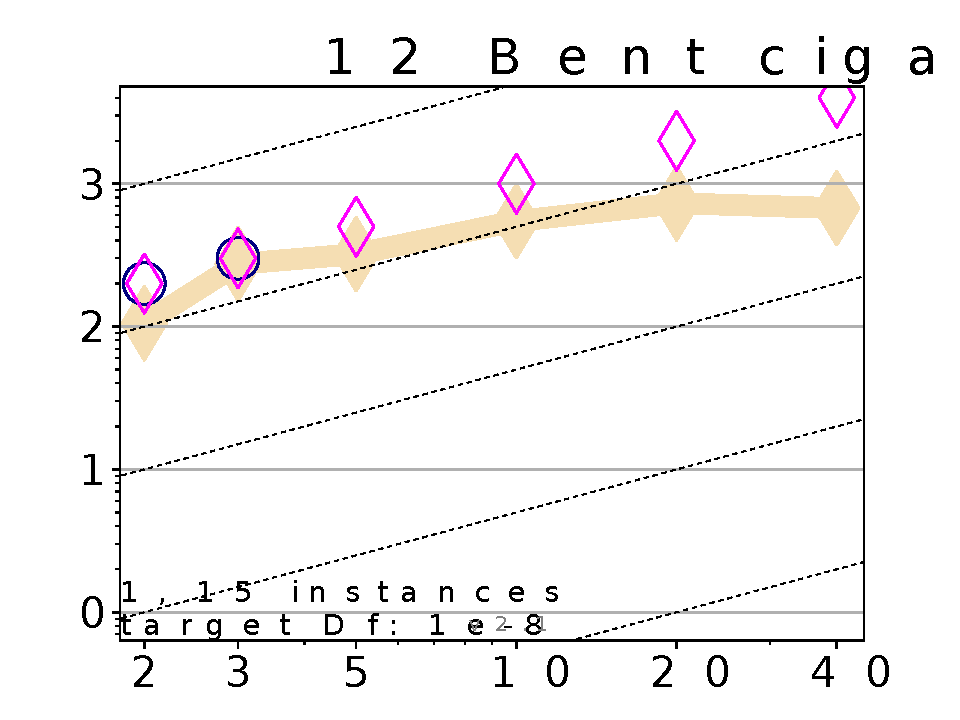
\includegraphics[width=0.238\textwidth, trim= 1.8cm 0.8cm 0.5cm 0.5cm, clip]{ppfigs_f012}\\
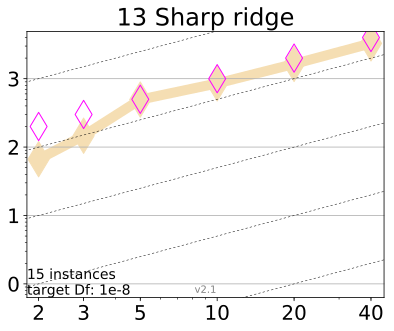
\includegraphics[width=0.253\textwidth, trim= 0.7cm 0.8cm 0.5cm 0.5cm, clip]{ppfigs_f013}&
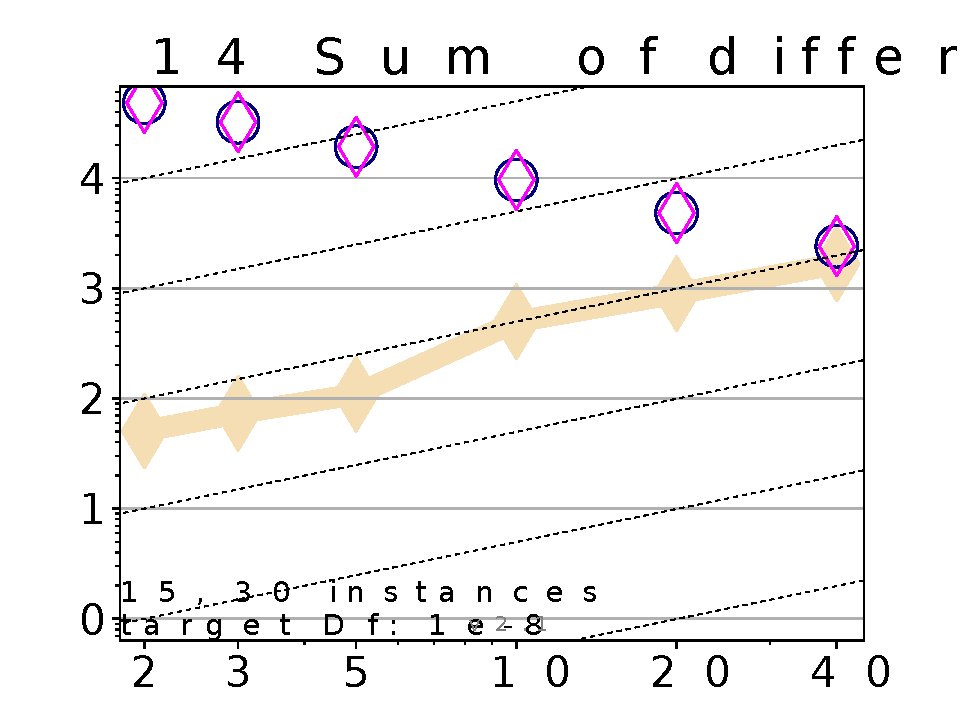
\includegraphics[width=0.238\textwidth, trim= 1.8cm 0.8cm 0.5cm 0.5cm, clip]{ppfigs_f014}&
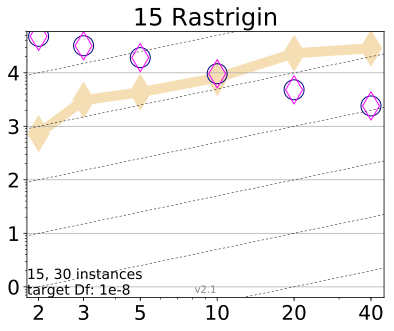
\includegraphics[width=0.238\textwidth, trim= 1.8cm 0.8cm 0.5cm 0.5cm, clip]{ppfigs_f015}&
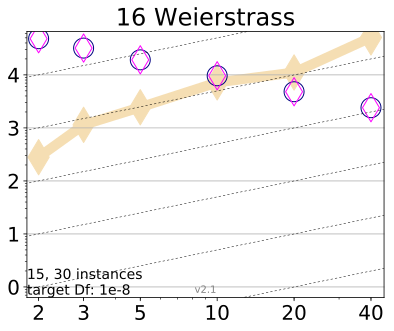
\includegraphics[width=0.238\textwidth, trim= 1.8cm 0.8cm 0.5cm 0.5cm, clip]{ppfigs_f016}\\
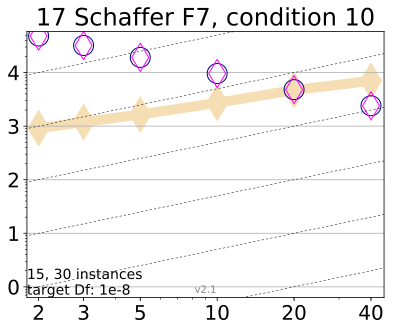
\includegraphics[width=0.253\textwidth, trim= 0.7cm 0.8cm 0.5cm 0.5cm, clip]{ppfigs_f017}&
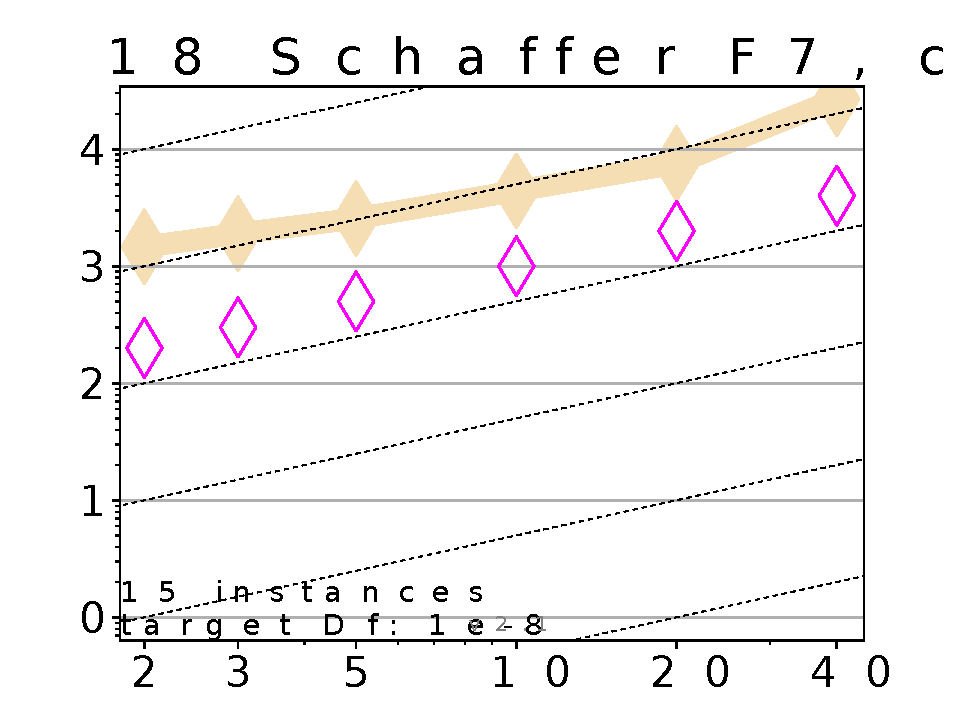
\includegraphics[width=0.238\textwidth, trim= 1.8cm 0.8cm 0.5cm 0.5cm, clip]{ppfigs_f018}&
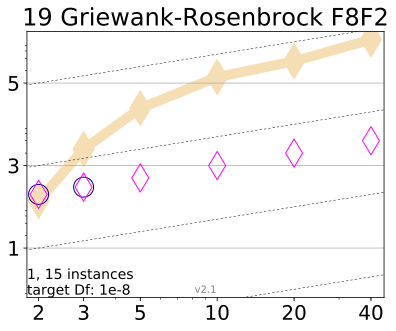
\includegraphics[width=0.238\textwidth, trim= 1.8cm 0.8cm 0.5cm 0.5cm, clip]{ppfigs_f019}&
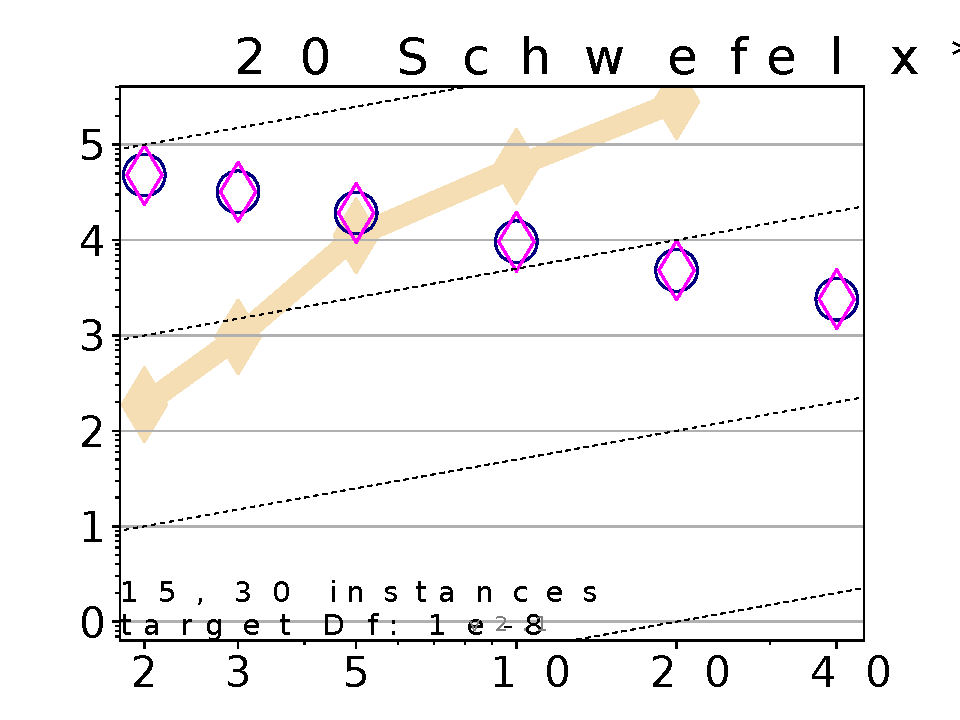
\includegraphics[width=0.238\textwidth, trim= 1.8cm 0.8cm 0.5cm 0.5cm, clip]{ppfigs_f020}\\
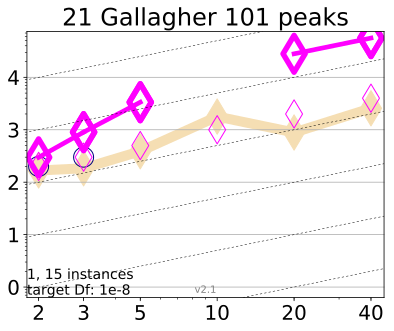
\includegraphics[width=0.253\textwidth, trim= 0.7cm 0.0cm 0.5cm 0.5cm, clip]{ppfigs_f021}&
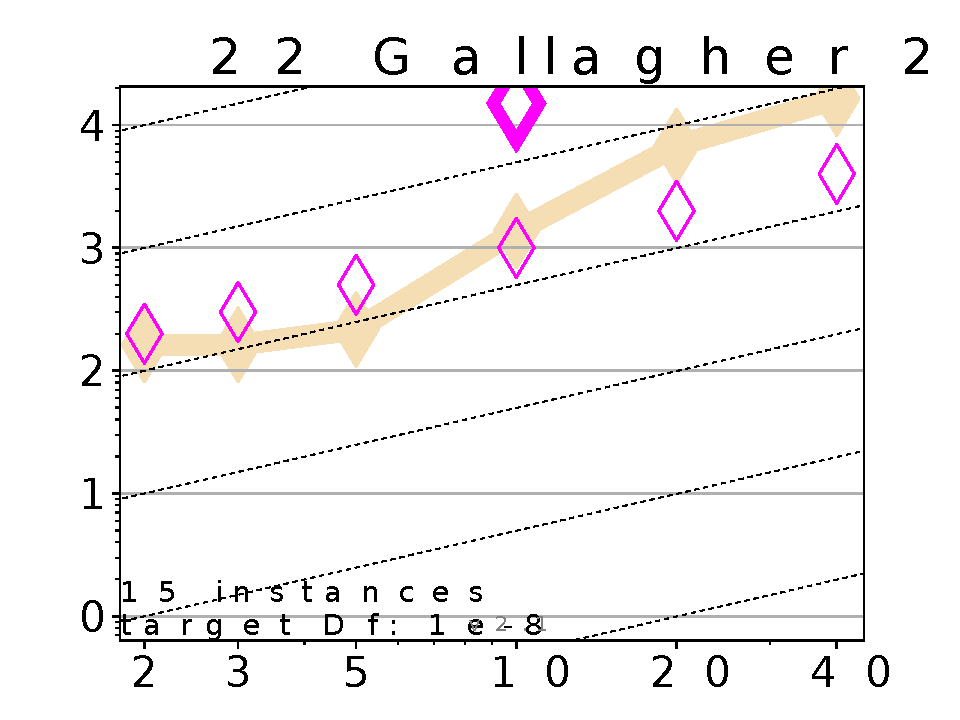
\includegraphics[width=0.238\textwidth, trim= 1.8cm 0.0cm 0.5cm 0.5cm, clip]{ppfigs_f022}&
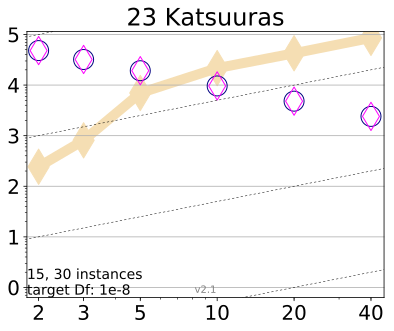
\includegraphics[width=0.238\textwidth, trim= 1.8cm 0.0cm 0.5cm 0.5cm, clip]{ppfigs_f023}&
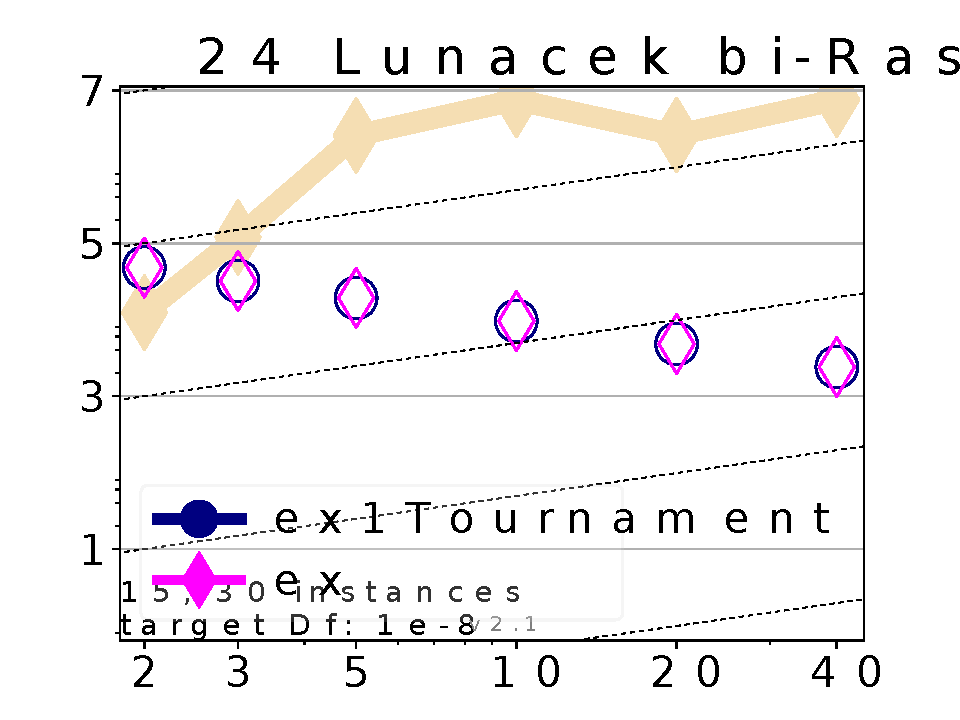
\includegraphics[width=0.238\textwidth, trim= 1.8cm 0.0cm 0.5cm 0.5cm, clip]{ppfigs_f024}
\end{tabular}
\vspace*{-0.2cm}
\caption[Expected running time divided by dimension versus dimension]{
\label{fig:scaling}
\bbobppfigslegend{$f_1$ and $f_{24}$}.  % note: \algorithmA and \algorithmB can be defined above
}
% 
\end{figure*}



%%%%%%%%%%%%%%%%%%%%%%%%%%%%%%%%%%%%%%%%%%%%%%%%%%%%%%%%%%%%%%%%%%%%%%%%%%%%%%%
%%%%%%%%%%%%%%%%%%%%%%%%%%%%%%%%%%%%%%%%%%%%%%%%%%%%%%%%%%%%%%%%%%%%%%%%%%%%%%%
 
% Scatter plots per function.

%%%%%%%%%%%%%%%%%%%%%%%%%%%%%%%%%%%%%%%%%%%%%%%%%%%%%%%%%%%%%%%%%%%%%%%%%%%%%%%

%%%%%%%%%%%%%%%%%%%%%%%%%%%%%%%%%%%%%%%%%%%%%%%%%%%%%%%%%%%%%%%%%%%%%%%%%%%%%%%
%%%%%%%%%%%%%%%%%%%%%%%%%%%%%%%%%%%%%%%%%%%%%%%%%%%%%%%%%%%%%%%%%%%%%%%%%%%%%%%
\newcommand{\rot}[2][2.5]{
  \hspace*{-3.5\baselineskip}%
  \begin{rotate}{90}\hspace{#1em}#2
  \end{rotate}}
%%%%%%%%%%%%%%%%%%%%%%%%%%%%%%%%%%%%%%%%%%%%%%%%%%%%%%%%%%%%%%%%%%%%%%%%%%%%%%%
%%%%%%%%%%%%%%%%%%%%%%%%%%%%%%%%%%%%%%%%%%%%%%%%%%%%%%%%%%%%%%%%%%%%%%%%%%%%%%%

\begin{figure*}
\begin{tabular}{*{4}{@{}c@{}}}
\begin{turn}{90}\parbox{0.21\textwidth}{\hfill\sf 1 Sphere\hfill~}\end{turn}
    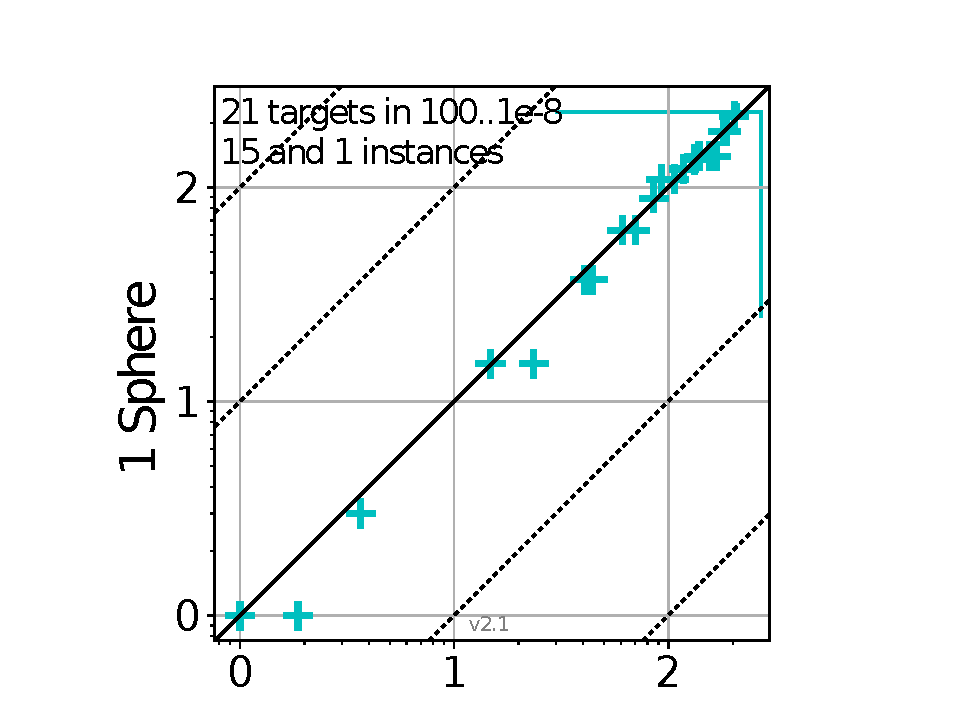
\includegraphics[height=0.21\textwidth, trim= 37mm 0mm 20mm 9mm, clip]{ppscatter_f001}&
\begin{turn}{90}\parbox{0.21\textwidth}{\hfill\sf 2 Ellipsoid separable\hfill~}\end{turn} 
    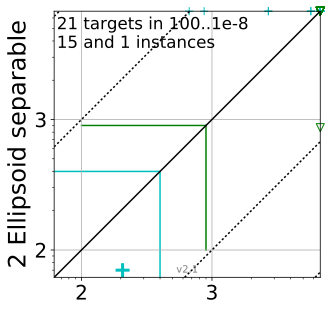
\includegraphics[height=0.21\textwidth, trim= 37mm 0mm 20mm 9mm, clip]{ppscatter_f002}&
\begin{turn}{90}\parbox{0.21\textwidth}{\hfill\sf 3 Rastrigin separable\hfill~}\end{turn} 
    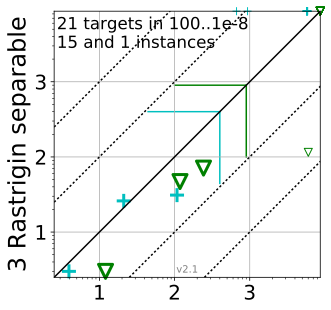
\includegraphics[height=0.21\textwidth, trim= 37mm 0mm 20mm 9mm, clip]{ppscatter_f003}&
\begin{turn}{90}\parbox{0.21\textwidth}{\hfill\sf 4 Skew Rastrigin-Bueche\hfill~}\end{turn} 
    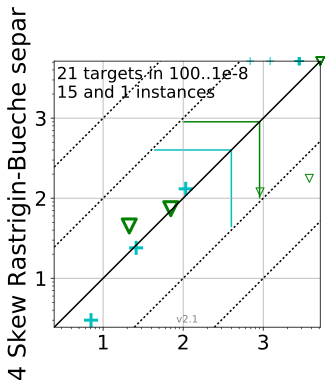
\includegraphics[height=0.21\textwidth, trim= 37mm 0mm 20mm 9mm, clip]{ppscatter_f004}\\[-2.2ex]
\begin{turn}{90}\parbox{0.21\textwidth}{\hfill\sf 5 Linear slope \hfill~}\end{turn} 
    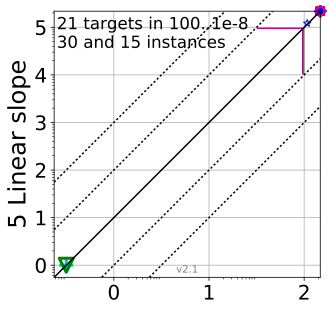
\includegraphics[height=0.21\textwidth, trim= 37mm 0mm 20mm 9mm, clip]{ppscatter_f005}&
\begin{turn}{90}\parbox{0.21\textwidth}{\hfill\sf 6 Attractive sector \hfill~}\end{turn} 
    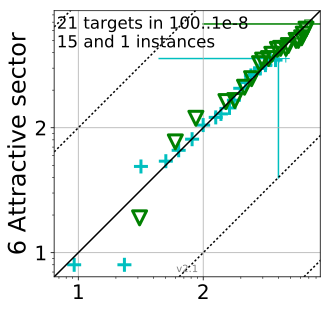
\includegraphics[height=0.21\textwidth, trim= 37mm 0mm 20mm 9mm, clip]{ppscatter_f006}&
\begin{turn}{90}\parbox{0.21\textwidth}{\hfill\sf 7 Step-ellipsoid \hfill~}\end{turn} 
    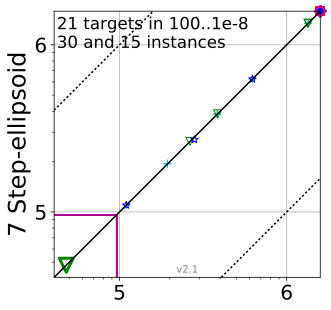
\includegraphics[height=0.21\textwidth, trim= 37mm 0mm 20mm 9mm, clip]{ppscatter_f007}&
\begin{turn}{90}\parbox{0.21\textwidth}{\hfill\sf 8 Rosenbrock original \hfill~}\end{turn} 
    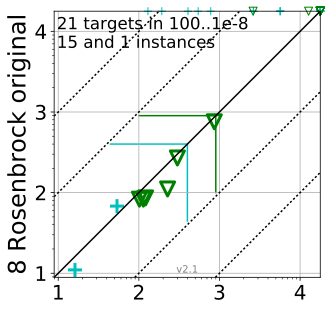
\includegraphics[height=0.21\textwidth, trim= 37mm 0mm 20mm 9mm, clip]{ppscatter_f008}\\[-2.2ex]
\begin{turn}{90}\parbox{0.21\textwidth}{\hfill\sf 9 Rosenbrock rotated \hfill~}\end{turn} 
    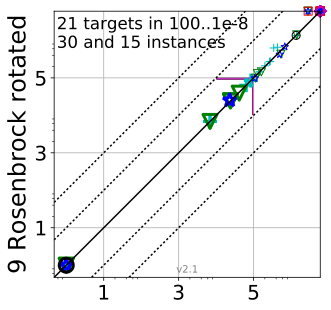
\includegraphics[height=0.21\textwidth, trim= 37mm 0mm 20mm 9mm, clip]{ppscatter_f009}&
\begin{turn}{90}\parbox{0.21\textwidth}{\hfill\sf 10 Ellipsoid \hfill~}\end{turn} 
    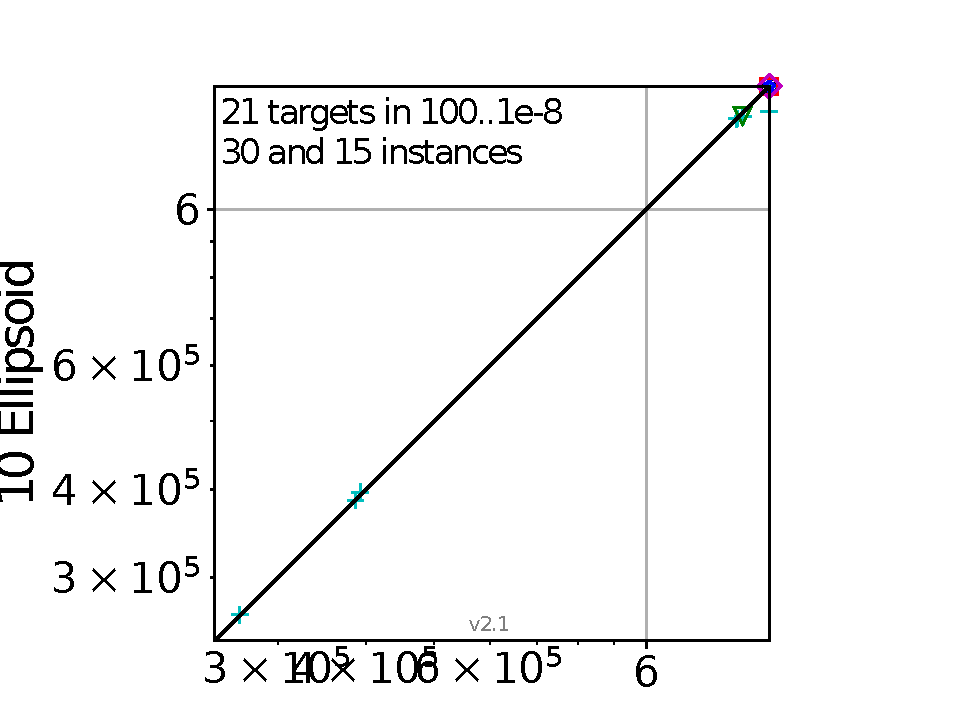
\includegraphics[height=0.21\textwidth, trim= 37mm 0mm 20mm 9mm, clip]{ppscatter_f010}&
\begin{turn}{90}\parbox{0.21\textwidth}{\hfill\sf 11 Discus \hfill~}\end{turn} 
    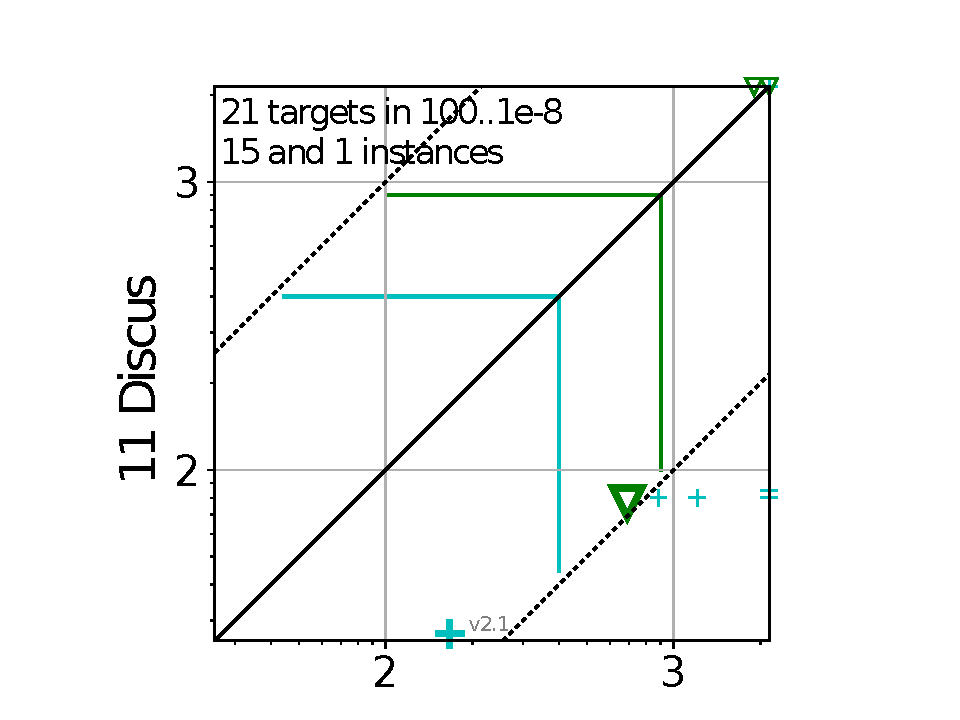
\includegraphics[height=0.21\textwidth, trim= 37mm 0mm 20mm 9mm, clip]{ppscatter_f011}&
\begin{turn}{90}\parbox{0.21\textwidth}{\hfill\sf 12 Bent cigar \hfill~}\end{turn} 
    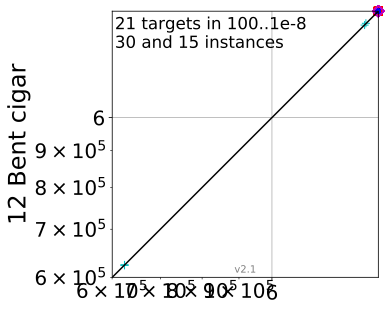
\includegraphics[height=0.21\textwidth, trim= 37mm 0mm 20mm 9mm, clip]{ppscatter_f012}\\[-2.2ex]
\begin{turn}{90}\parbox{0.21\textwidth}{\hfill\sf 13 Sharp ridge \hfill~}\end{turn} 
    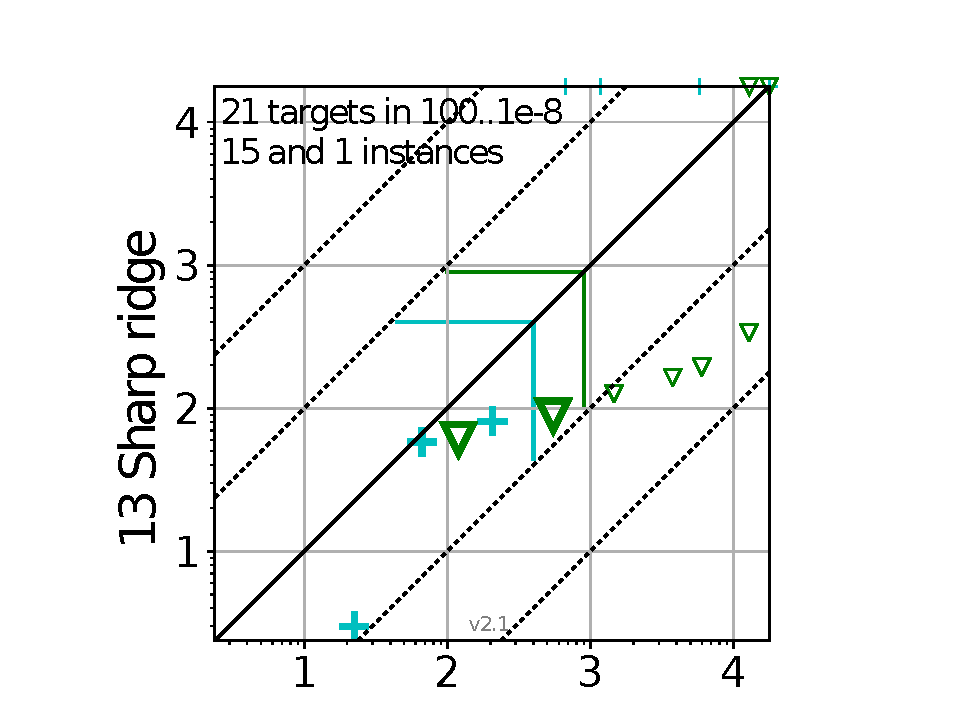
\includegraphics[height=0.21\textwidth, trim= 37mm 0mm 20mm 9mm, clip]{ppscatter_f013}&
\begin{turn}{90}\parbox{0.21\textwidth}{\hfill\sf~~14 Sum of diff.\ powers \hfill~}\end{turn} 
    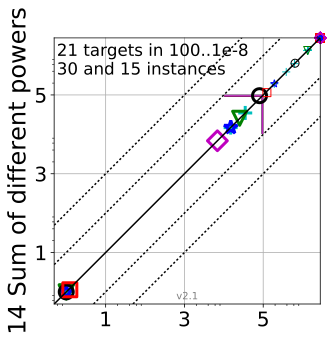
\includegraphics[height=0.21\textwidth, trim= 37mm 0mm 20mm 9mm, clip]{ppscatter_f014}&
\begin{turn}{90}\parbox{0.21\textwidth}{\hfill\sf 15 Rastrigin \hfill~}\end{turn} 
    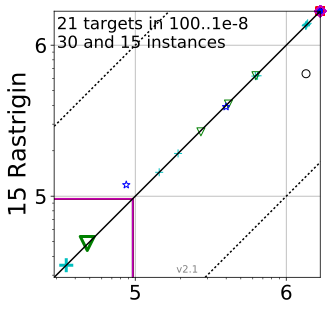
\includegraphics[height=0.21\textwidth, trim= 37mm 0mm 20mm 9mm, clip]{ppscatter_f015}&
\begin{turn}{90}\parbox{0.21\textwidth}{\hfill\sf 16 Weierstrass \hfill~}\end{turn} 
    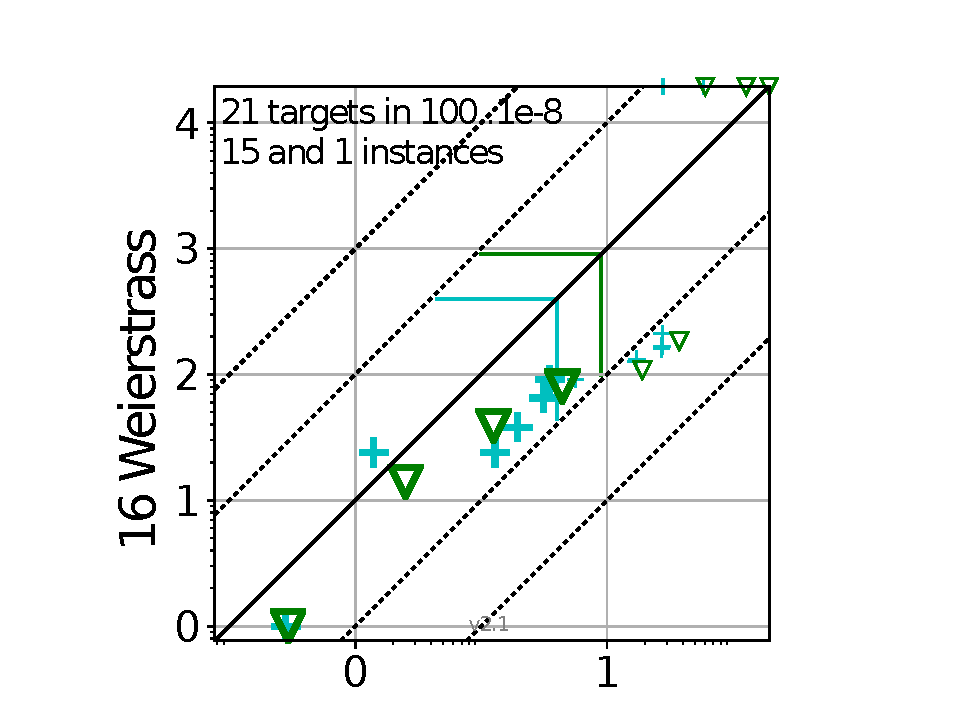
\includegraphics[height=0.21\textwidth, trim= 37mm 0mm 20mm 9mm, clip]{ppscatter_f016}\\[-2.2ex]
\begin{turn}{90}\parbox{0.21\textwidth}{\hfill\sf 17 Schaffer F7, cond.10 \hfill~}\end{turn} 
    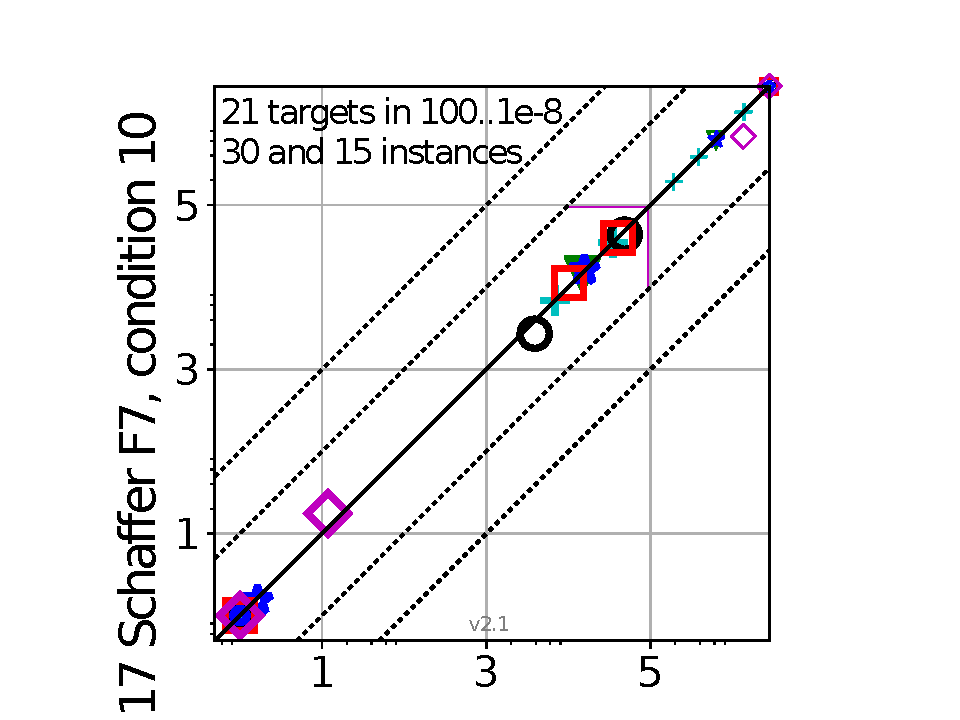
\includegraphics[height=0.21\textwidth, trim= 37mm 0mm 20mm 9mm, clip]{ppscatter_f017}&
\begin{turn}{90}\parbox{0.21\textwidth}{\hfill\sf 18 Schaffer F7, cond.1000 \hfill~}\end{turn} 
    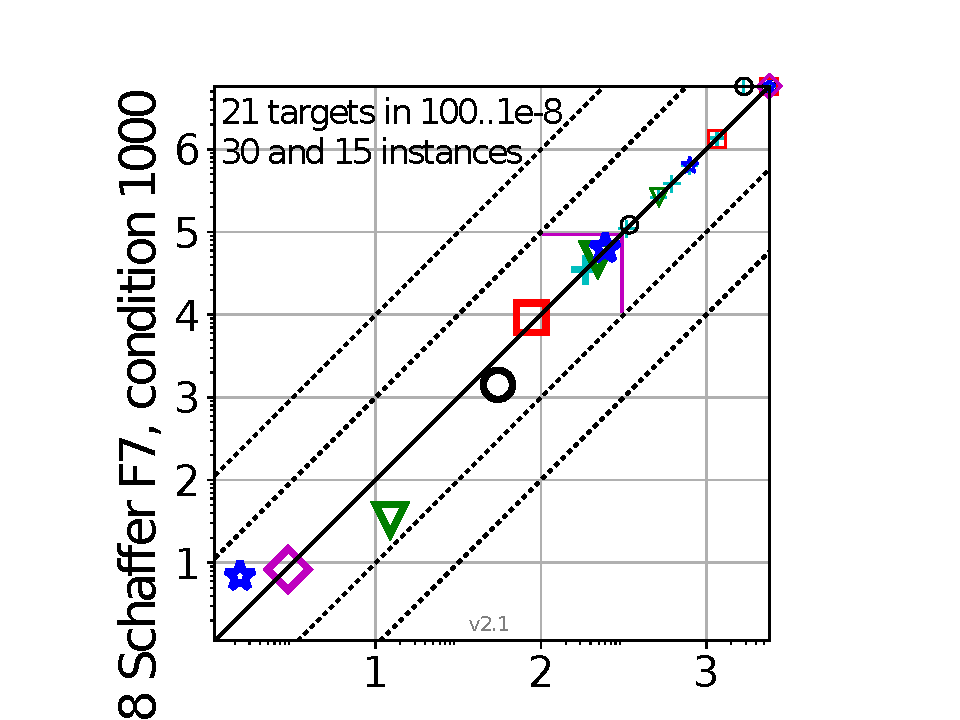
\includegraphics[height=0.21\textwidth, trim= 37mm 0mm 20mm 9mm, clip]{ppscatter_f018}&
\begin{turn}{90}\parbox{0.21\textwidth}{\hfill\sf 19 Griewank-Rosenbrock \hfill~}\end{turn} 
    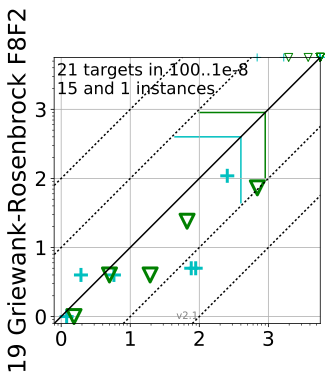
\includegraphics[height=0.21\textwidth, trim= 37mm 0mm 20mm 9mm, clip]{ppscatter_f019}&
\begin{turn}{90}\parbox{0.21\textwidth}{\hfill\sf 20 Schwefel x*sin(x) \hfill~}\end{turn} 
    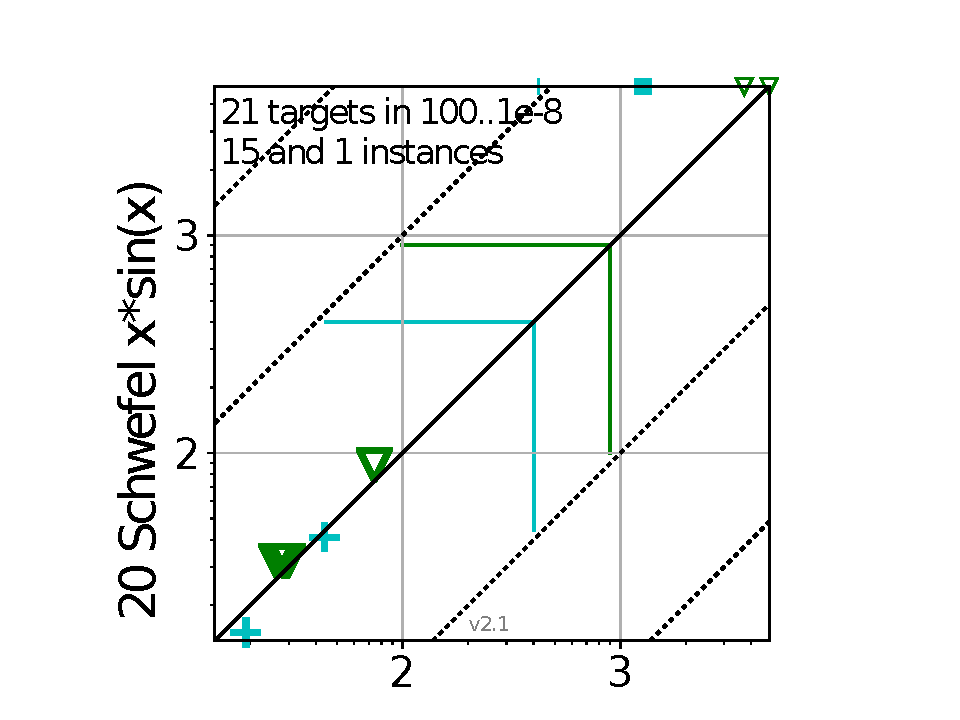
\includegraphics[height=0.21\textwidth, trim= 37mm 0mm 20mm 9mm, clip]{ppscatter_f020}\\[-2.2ex]
\begin{turn}{90}\parbox{0.21\textwidth}{\hfill\sf 21 Gallagher 101 peaks \hfill~}\end{turn} 
    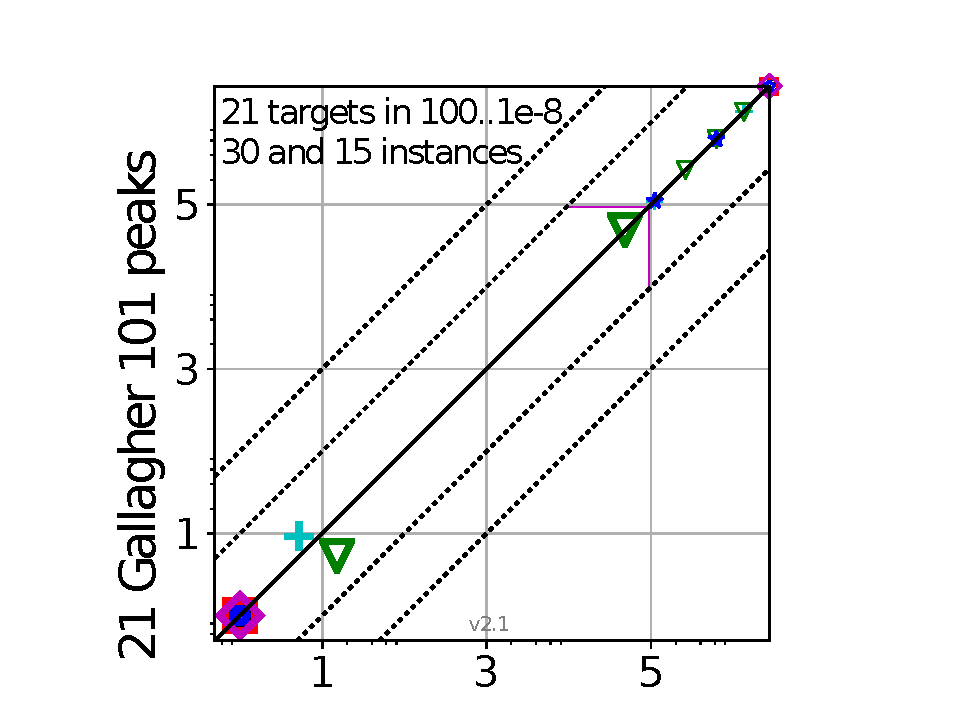
\includegraphics[height=0.21\textwidth, trim= 37mm 0mm 20mm 9mm, clip]{ppscatter_f021}&
\begin{turn}{90}\parbox{0.21\textwidth}{\hfill\sf 22 Gallagher 21 peaks \hfill~}\end{turn} 
    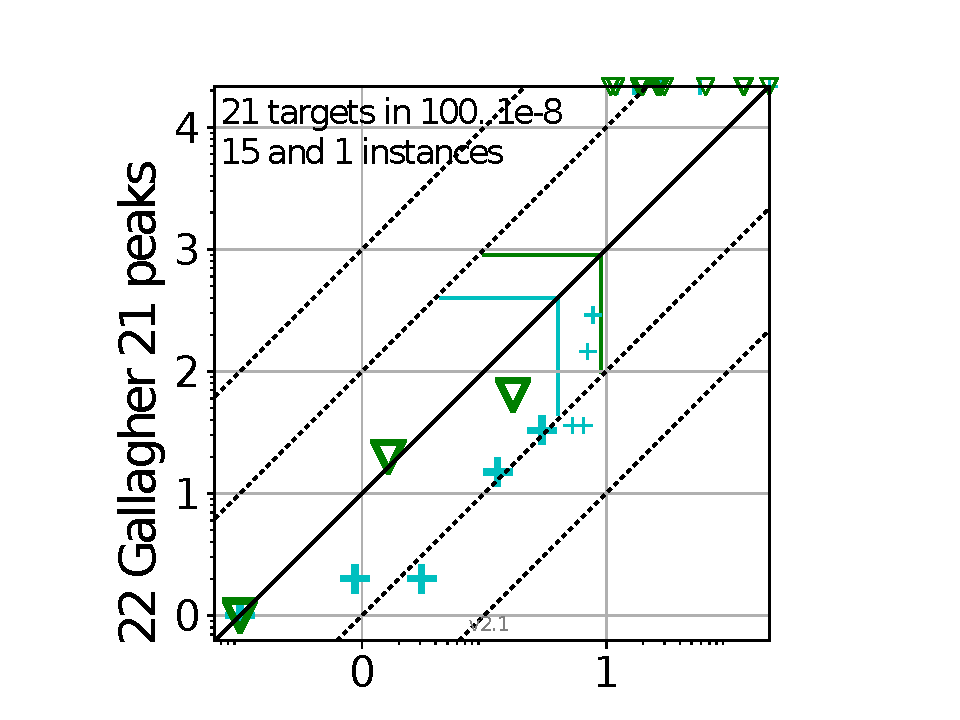
\includegraphics[height=0.21\textwidth, trim= 37mm 0mm 20mm 9mm, clip]{ppscatter_f022}&
\begin{turn}{90}\parbox{0.21\textwidth}{\hfill\sf 23 Katsuuras \hfill~}\end{turn} 
    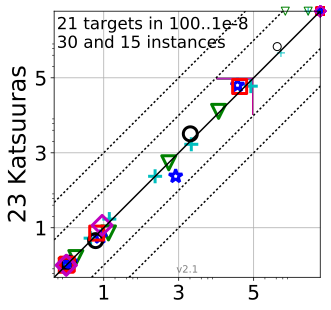
\includegraphics[height=0.21\textwidth, trim= 37mm 0mm 20mm 9mm, clip]{ppscatter_f023}&
\begin{turn}{90}\parbox{0.21\textwidth}{\hfill\sf 24 Lunacek bi-Rastrigin \hfill~}\end{turn} 
    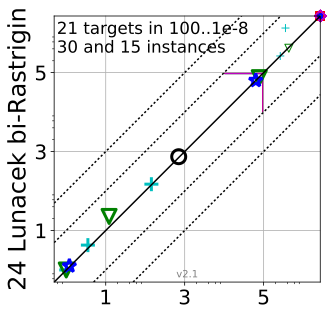
\includegraphics[height=0.21\textwidth, trim= 37mm 0mm 20mm 9mm, clip]{ppscatter_f024}
\end{tabular}
\caption{\label{fig:scatterplots}
\bbobppscatterlegend{$f_1$--$f_{24}$}
}
\end{figure*}


%%%%%%%%%%%%%%%%%%%%%%%%%%%%%%%%%%%%%%%%%%%%%%%%%%%%%%%%%%%%%%%%%%%%%%%%%%%%%%%
%%%%%%%%%%%%%%%%%%%%%%%%%%%%%%%%%%%%%%%%%%%%%%%%%%%%%%%%%%%%%%%%%%%%%%%%%%%%%%%
 
% Empirical cumulative distribution functions (ECDFs) per function group.

%%%%%%%%%%%%%%%%%%%%%%%%%%%%%%%%%%%%%%%%%%%%%%%%%%%%%%%%%%%%%%%%%%%%%%%%%%%%%%%
\begin{figure*}
 \begin{tabular}{l@{\hspace*{-0.025\textwidth}}l|l@{\hspace*{-0.025\textwidth}}l}
 \multicolumn{2}{c}{5-D} & \multicolumn{2}{c}{20-D} \\
 \rot{separable fcts}
 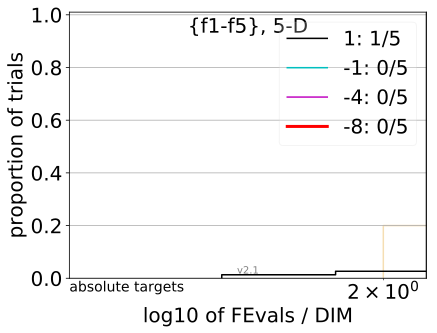
\includegraphics[width=0.268\textwidth,trim=     0mm 0mm 0mm 15mm, clip]{pprldistr_05D_separ} & 
 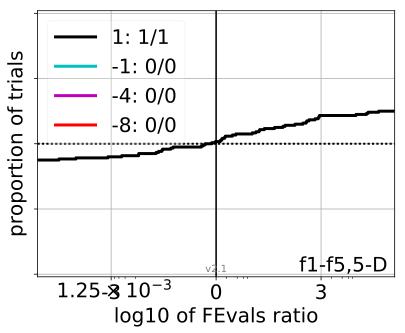
\includegraphics[width=0.2375\textwidth,trim=2.3cm 0mm 0mm 15mm, clip]{pplogabs_05D_separ} &
 \includegraphics[width=0.268\textwidth,trim=     0mm 0mm 0mm 15mm, clip]{pprldistr_20D_separ} &
 \includegraphics[width=0.2375\textwidth,trim=2.3cm 0mm 0mm 15mm, clip]{pplogabs_20D_separ} \\
 \rot[2]{moderate fcts}
 \includegraphics[width=0.268\textwidth,trim=     0mm 0mm 0mm 15mm, clip]{pprldistr_05D_lcond} & 
 \includegraphics[width=0.2375\textwidth,trim=2.3cm 0mm 0mm 15mm, clip]{pplogabs_05D_lcond} &
 \includegraphics[width=0.268\textwidth,trim=     0mm 0mm 0mm 15mm, clip]{pprldistr_20D_lcond} & 
 \includegraphics[width=0.2375\textwidth,trim=2.3cm 0mm 0mm 15mm, clip]{pplogabs_20D_lcond}\\
 \rot[1.3]{ill-conditioned fcts}
 \includegraphics[width=0.268\textwidth,trim=     0mm 0mm 0mm 15mm, clip]{pprldistr_05D_hcond} & 
 \includegraphics[width=0.2375\textwidth,trim=2.3cm 0mm 0mm 15mm, clip]{pplogabs_05D_hcond} &
 \includegraphics[width=0.268\textwidth,trim=     0mm 0mm 0mm 15mm, clip]{pprldistr_20D_hcond} &
 \includegraphics[width=0.2375\textwidth,trim=2.3cm 0mm 0mm 15mm, clip]{pplogabs_20D_hcond} \\
 \rot[1.6]{multi-modal fcts}
 \includegraphics[width=0.268\textwidth,trim=     0mm 0mm 0mm 15mm, clip]{pprldistr_05D_multi} & 
 \includegraphics[width=0.2375\textwidth,trim=2.3cm 0mm 0mm 15mm, clip]{pplogabs_05D_multi} &
 \includegraphics[width=0.268\textwidth,trim=     0mm 0mm 0mm 15mm, clip]{pprldistr_20D_multi} &
 \includegraphics[width=0.2375\textwidth,trim=2.3cm 0mm 0mm 15mm, clip]{pplogabs_20D_multi} \\
 \rot[1.0]{weak structure fcts}
 \includegraphics[width=0.268\textwidth,trim=     0mm 0mm 0mm 15mm, clip]{pprldistr_05D_mult2} & 
 \includegraphics[width=0.2375\textwidth,trim=2.3cm 0mm 0mm 15mm, clip]{pplogabs_05D_mult2} &
 \includegraphics[width=0.268\textwidth,trim=     0mm 0mm 0mm 15mm, clip]{pprldistr_20D_mult2} & 
 \includegraphics[width=0.2375\textwidth,trim=2.3cm 0mm 0mm 15mm, clip]{pplogabs_20D_mult2}\\
 \rot{all functions}
 \includegraphics[width=0.268\textwidth,trim=0cm 0mm 0mm 15mm, clip]{pprldistr_05D_noiselessall} & 
 \includegraphics[width=0.2375\textwidth,trim=2.3cm 0mm 0mm 15mm, clip]{pplogabs_05D_noiselessall} &
 \includegraphics[width=0.268\textwidth,trim=0cm 0mm 0mm 15mm, clip]{pprldistr_20D_noiselessall} &
 \includegraphics[width=0.2375\textwidth,trim=2.3cm 0mm 0mm 15mm, clip]{pplogabs_20D_noiselessall}
 \end{tabular}
\vspace*{-0.2cm}
 \caption{\label{fig:RLDs}
 \bbobpprldistrlegendtwo{}
 }
\end{figure*}


%%%%%%%%%%%%%%%%%%%%%%%%%%%%%%%%%%%%%%%%%%%%%%%%%%%%%%%%%%%%%%%%%%%%%%%%%%%%%%%
%%%%%%%%%%%%%%%%%%%%%%%%%%%%%%%%%%%%%%%%%%%%%%%%%%%%%%%%%%%%%%%%%%%%%%%%%%%%%%%
 
% Table showing the average runtime (aRT in number of function
% evaluations) divided by the best aRT measured during BBOB-2009 (given in the
% first row of each cell) for functions $f_1$--$f_{24}$.

%%%%%%%%%%%%%%%%%%%%%%%%%%%%%%%%%%%%%%%%%%%%%%%%%%%%%%%%%%%%%%%%%%%%%%%%%%%%%%%
\begin{table*}
\centering
\hfill5-D\hfill20-D\hfill~\\[1ex]
\tiny
\mbox{
\input{\bbobdatapath pptable2_05D_noiselessall}\hfill%
\input{\bbobdatapath pptable2_20D_noiselessall}}
\caption{\label{tab:aRTs}
\bbobpptablestwolegend{dimensions $5$ (left) and $20$ (right)}{48}
}
\end{table*}



%%%%%%%%%%%%%%%%%%%%%%%%%%%%%%%%%%%%%%%%%%%%%%%%%%%%%%%%%%%%%%%%%%%%%%%%%%%%%%%

\bibliographystyle{ACM-Reference-Format}
\bibliography{bbob}  % bbob.bib is the name of the Bibliography in this case

\clearpage % otherwise the last figure might be missing



\end{document}

%%%%%%%%%%%%%%%%%%%%%%%%%%%%%%%%%%%%%%%%%%%%%%%%%%%%%%%%%%%%%%%%%%%%%%%%%%%%%%%%%%%%%%%%%%%
